\documentclass[11pt]{article}
%you can look for fun LaTeX packages to use hereasdf

\usepackage{amsmath}
\usepackage{amssymb}
\usepackage{fancyhdr}
\usepackage{amsthm}

\usepackage{graphicx}
\usepackage{dcolumn}
\usepackage{bm}

%fun commands for fun sets
%make sure to use these in math mode
\newcommand{\Z}{\mathbb{Z}}
\newcommand{\R}{\mathbb{R}}
\newcommand{\N}{\mathbb{N}}
\newcommand{\C}{\mathbb{C}}
\newcommand{\m}{\mathcal{M}}
\newcommand{\Tt}{\mathcal{T}}
\newcommand{\pa}{\partial}
\newcommand{\dD}{\mathcal{D}}
\newcommand{\E}{\mathbb{E}}



\oddsidemargin0cm
\topmargin-2cm    
\textwidth16.5cm   
\textheight23.5cm  

\newcommand{\question}[2] {\vspace{.25in} \hrule\vspace{0.5em}
\noindent{\bf #1: #2} \vspace{0.5em}
\hrule \vspace{.10in}}
\renewcommand{\part}[1] {\vspace{.10in} {\bf (#1)}}

\newcommand{\myname}{Alex Havrilla}
\newcommand{\myandrew}{alumhavr}
\newcommand{\myhwnum}{Hw 1}

\newtheorem{theorem}{Theorem}
\newtheorem{prop}{Prop}
\theoremstyle{remark}
\newtheorem{lemma}{Lemma}
\newtheorem{remark}{Remark}
\newtheorem{defi}{Def}
\newtheorem{apps}{Application}
\newtheorem{quest}{Question}
\newtheorem{ans}{Answer}
\newtheorem{interest}{Interesting}
\newtheorem{theme}{Theme}
\newtheorem{back}{Background}
\newtheorem{idea}{Idea}
\newtheorem{example}{Example}

\setlength{\parindent}{0pt}
\setlength{\parskip}{5pt plus 1pt}
 
\pagestyle{fancyplain}
\lhead{\fancyplain{}{\textbf{HW\myhwnum}}}      % Note the different brackets!
\rhead{\fancyplain{}{\myname\\ \myandrew}}
\chead{\fancyplain{}{\mycourse}}

\linespread{1.3}

\title{PDE and Data Analysis}

\begin{document}

\maketitle

\section{Introductions}

\textbf{TAG:} OptimalTransport

\begin{theme}
	The more assumptions you make on a measure the better approximation you can achieve
\end{theme}

\begin{interest}
	Shimaa is interested in stochastic BDEs. Wes interested in foundations of machine learning.
\end{interest}

\begin{theme}
	Look at a measure as some kind of energy landscape and the transport map as the process of rearranging mass.
\end{theme}

\begin{remark}
	Often transportation cost is $|x-y|^p$. 
\end{remark}

\begin{remark}
	Optimal transport minimizes transportation cost.
\end{remark}

\begin{theme}
	Goal is to find weaker problem which provides good solution to wider class of subproblems.
\end{theme}

\section{Optimal Transport}

\textbf{TAG:} OptimalTransport

\begin{remark}
	Villani's Optimal Transport: New and Old
	\begin{verbatim}
		https://ljk.imag.fr/membres/Emmanuel.Maitre/lib/exe/fetch.php?media=b07.stflour.pdf
	\end{verbatim}
	Presented from a probabilistic perspective.
\end{remark}

\begin{remark}
	Via CoV, condition for transport map:
	\begin{align*}
		\rho(x) = \eta(T(x)) |det(DT(x))|
	\end{align*}
\end{remark}

\begin{prop}
	Change of variables formula justified via above:
	\begin{align*}
		\int_Y f(y) d\nu(y) = \int_X f(T(x))d\mu(x)
	\end{align*}
\end{prop}

\begin{quest}
	When does measure preserving map even exist between $\mu$ on X and $\nu$ on Y. 
\end{quest}

\begin{example}
	Consider to the above the non-example $\mu(x) = 1$, $\nu(y_1) = \nu(y_2) = 1/2$. 
\end{example}

\begin{remark}
	Transport plan is generalization of transport map that has the source and target measures as its marginals. If  we have a transport map then $(I \times T)_{\sharp}\mu$ is a transport plan. Effectively pushing measure onto graph of T(note I is identity). 
\end{remark}

\begin{quest}
	Why does $\mu \times \nu$ not always work? 
\end{quest}

\begin{ans}
	It does.
\end{ans}

\begin{remark}
	Optimal Transport cost in terms of plans is always well defined since a plan exists and infimum is always a min(this is the Kantorovich formulation, first one is monge formulation)
	\begin{align*}
		C(\pi) = \int_{X \times Y} c(x,y) d\pi(x,y) = \int_{X \times Y} c(x,y) d(I \times T)_{\sharp} \mu = \int_X c(x,T(x))d\mu(x)
	\end{align*}
\end{remark}

\begin{quest}
	In kantorovich, how do we know infimum is always min?
\end{quest}

\subsection{Calculus of Variations}

\textbf{TAG:} VariationalCalculus

\begin{prop}
	Norms are lsc
\end{prop}

\begin{example}
	Picture of lsc function:
	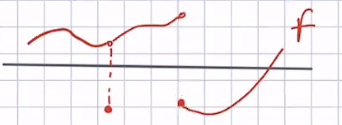
\includegraphics[width=250px]{C:/Users/Alex/Desktop/Notes/Spring 2021/pics/lsc.png}
\end{example}

\begin{prop}
	lsc functions achieve mins on compact sets
\end{prop}

\begin{proof}
	Let m inf. Let $x_n$ s.t. $f(x_n) \to m$. Sequential compactness gives us subsequence so that limit x stays in X. Thus $f(x)$ is minimizer since it must be smaller than all other valuations. 
\end{proof}

\begin{theorem}
	If X,Y compact and $c : X \times Y\to R$ then the kantorovich formulation has a solution
\end{theorem}

\begin{proof}
	\textbf{Proof using direct method of calculus of variations}

	$T_c : P(X\times Y) \to R$ is cts. w.r.t narrow convergence so $\int c \gamma = T_c(\gamma)$. Since $P(X \times Y)$ is tight and thus compact w.r.t narrow conv. Then if $\gamma_n \in \Pi(\mu,\nu)$ is a minimizing seq. then we have conv. subseq in product $P(X \times Y)$ for some $\gamma$. Need  $\gamma \in \Pi$. Doable by evauating marginals directly via  defintions above
\end{proof}

\begin{theme}
	We study measures by looking at test functions, which all for equality. Key idea is to look for notions which allow us to gai equality.
\end{theme}

\begin{prop}
	$\Pi(\mu,\nu)$ is convex.
\end{prop}

\end{document}

